\begin{figure}[t]
    \centering
    % 4K
    \begin{subfigure}{\textwidth}
        \centering
        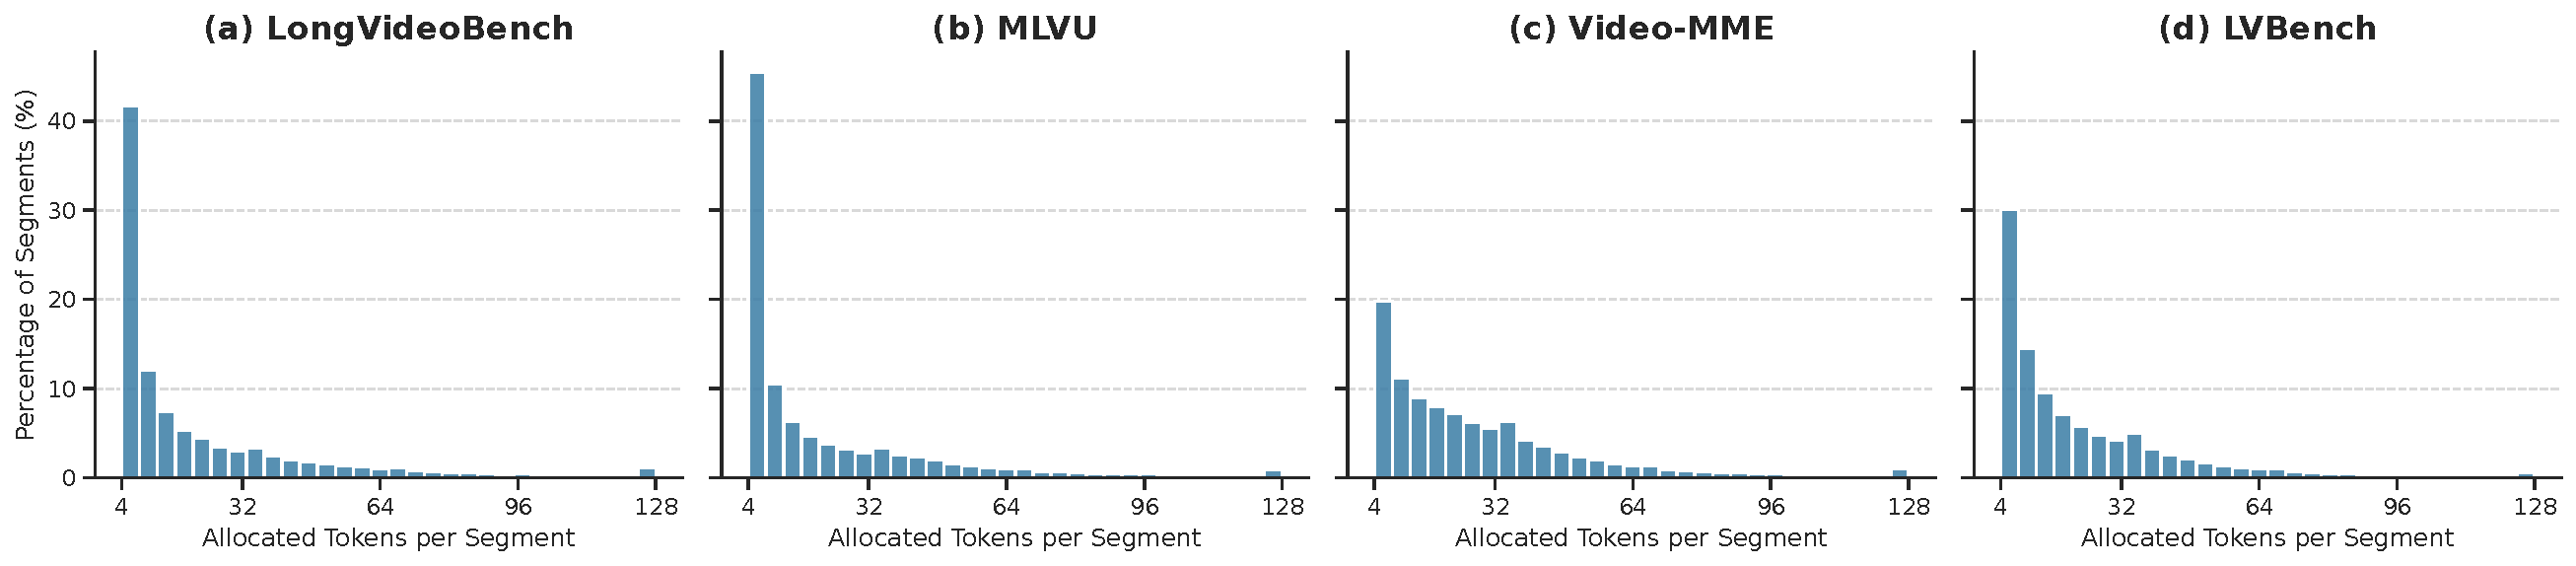
\includegraphics[width=0.95\linewidth]{supp/fig/token_overall_allocation_4k.pdf}
        \vspace{-0.5em}
    \end{subfigure}
    \\ \vspace{1em}
    % 8K
    \begin{subfigure}{\textwidth}
        \centering
        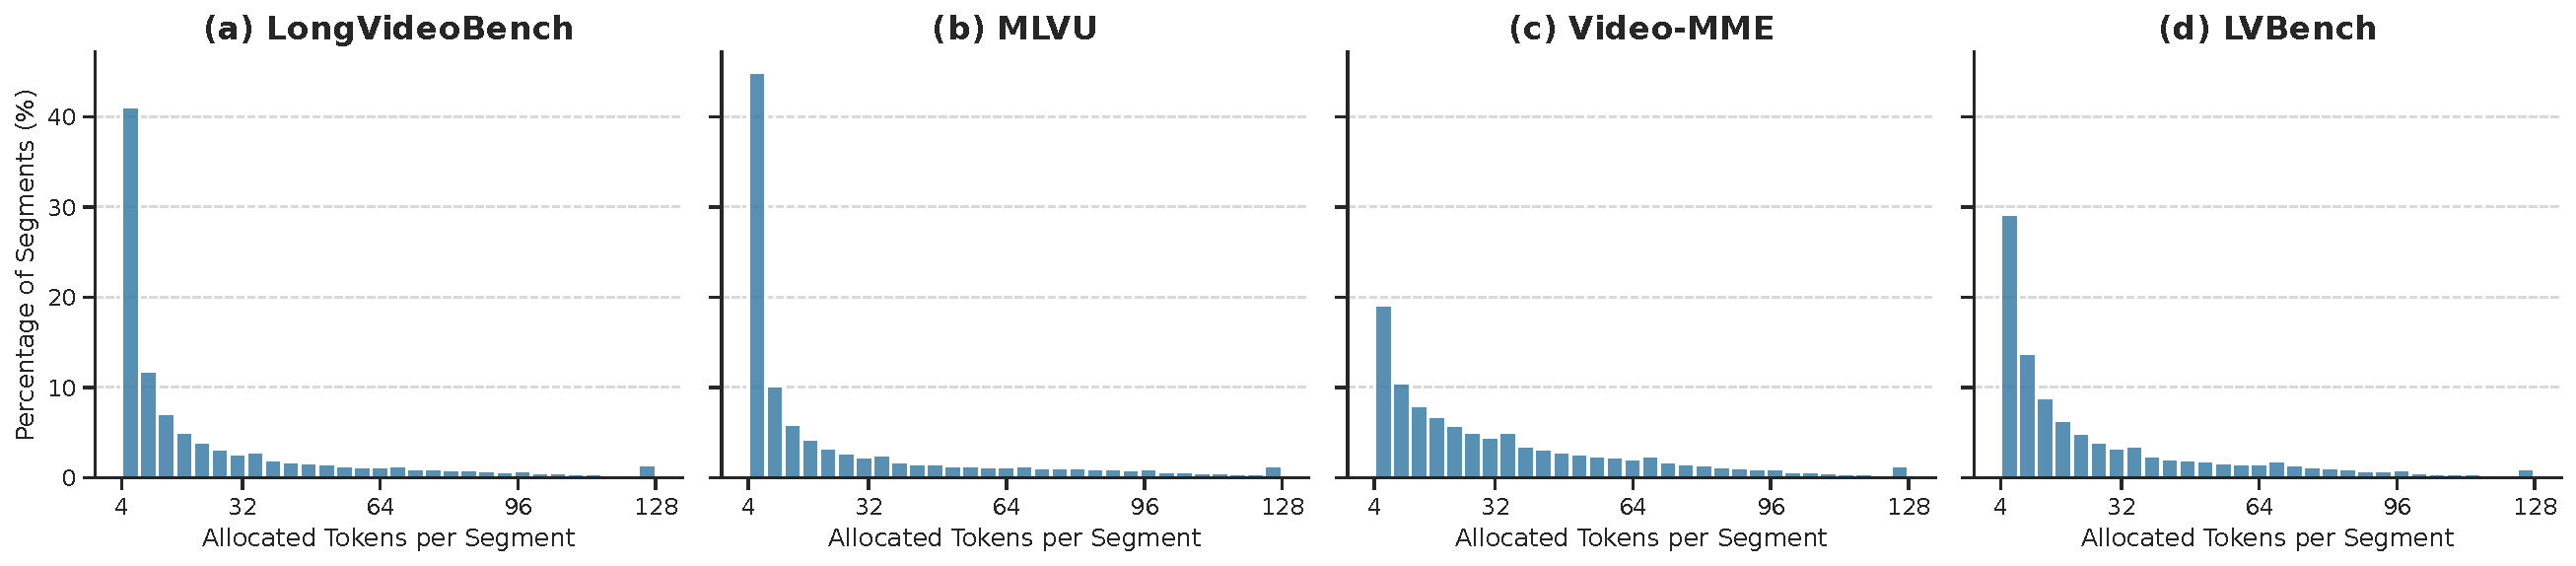
\includegraphics[width=0.95\linewidth]{supp/fig/token_overall_allocation_8k.pdf}
        \vspace{-0.5em}
    \end{subfigure}
    \caption{
        \textbf{Distribution of allocated tokens per segment.}
        \textbf{(Top)} 4K budget ($B=4096$); \textbf{(Bottom)} 8K budget ($B=8192$).
        Across four benchmarks, ATA consistently exhibits a strongly right-skewed, long-tailed allocation pattern. The majority of segments are compressed into very low-token representations, while a small fraction receives substantially higher allocations for query-aligned segments. Notably, this distribution pattern remains stable under different global budgets.
    }
    \label{fig:micro_dist}
\end{figure}